\documentclass[
  aps,
  reprint,
  twoside,
  showpacs,
  amsmath,
  amssymb,
  floatfix
]{revtex4-1}
\usepackage{graphicx}

%
% Todo list:
% done - Convergence study.  Discuss this in terms of the time scales
%   involved (especially the time it takes the ions to travel an inter-
%   ion distance
% - Spectrum of axial phonon modes
%   . mode structures,
%   . temperatures/occupancies
% - Spectrum of in-plane phonon modes
%   . mode structures,
%   . temperatures/occupancies
% - Local ion spectra
% - Local ion mobility in steady state
% - Dynamics of crystal rearrangements
%   . Frequency with which they occur
%   . Where in the crystal do they occur
% - Impact of size of in-plane cooling beam on temperature and crystal
%   stability:
%   . Scan cooling beam stability
% - Impact of misalignment of in-plane cooling beam on crystal stability
%   . Scan misalignment
% need a figure that shows the overall setup of the experiment
%

\newcommand{\domcomment}[1]{{\tt #1}}

\begin{document}

\title{Dynamical simulations of phonon dynamics in ultra-cold ion
  crystals}
\author{D. Meiser}
\affiliation{
  Tech-X Corporation,
  5261 Arapahoe Ave. Ste A,
  Boulder, Colorado 80303, USA.}
\author{J. Britton}
\author{B. Sawyer}
\author{J. J. Bollinger}
\affiliation{NIST Boulder}
\maketitle


\section{Introduction}
\label{sec:introduction}


Ultra-cold ions in Penning traps are an extremely powerful experimental
platform for research in quantum information science and quantum
computing~\cite{QuantumComputing} and quantum information, quantum
simulation, and quantum metrology.  These systems have been used to
simulated complex, strongly correlated condensed matter systems and
quantum magnetic systems~\cite{IsingStuff}.

\domcomment{Also mention plasma physics problems that can be studied.
  Very strongly correlated plasma.}

Successful experiments in these areas critically depend on laser cooling
of the ions to near their motional ground state.  At these temperatures
the ions form a crystal that is the basis of e.g. the quantum simulation
experiments.  The next generation of experiments requires colder
temperatures (or rather more stable crystals).  That would allow single
site state preparation and single site readout, perhaps doing quantum
computation in Penning traps with much larger numbers of ions than
what's possible in Paul traps.

Simulation can provide very useful insight into the thermal ion
dynamics, rearrangements of the ions in the crystal, and the interplay
between these phenomena and the laser cooling and trap characteristics.  
\domcomment{Discuss some of the stuff that the Freericks group has done
with their simulations}

Here we present results from molecular dynamics simulations of the ion
motion in a Penning trap including laser cooling.  By including a
microscopic model of the laser cooling that includes damping and recoil
heating we are able to go beyond what's been done before.  We get the
temperature of the individual phonon modes and we can study the mobility
of the ions on a per site basis.  We can study the ion dynamics over a
wider range of trap geometries (greater aspect ratio, multi-plane
    crystals, etc.).  We can study the impact of misalignment of the
cooling lasers and we can study the crystal stability as a function of
the diameter of the cooling lasers.  More complex cooling geometries
(e.g. two counter-propagating cooling beams) can be studied easily,
providing valuable insight for potential future improvements of the
experiment.

Describe the major challenge in the theory of the laser cooling of th
in-plane motion.

In this paper...

\section{Numerical integration of ion dynamics}
\label{sec:integrators}

Our goal is a first principles, microscopic simulation of the ion
dynamics.  We have to account for the
following forces acting on the ions:
\domcomment{More detailed description of Penning trap needed.
  Reference to Freericks paper}
\begin{itemize}

\item Cyclotron motion in the axial magnetic field of approximately 5T.

\item Coulomb interactions between the ions.

\item Electro-static trapping potential and rotating-wall potential.

\item Laser cooling forces including damping and fluctuations.

\end{itemize}

In this section we describe our model for these forces and how we deal
with them numerically.


\subsection{Ion Hamiltonian}
\label{ssec:Hamiltonian}

Some of the forces are easier to express in the lab frame and some of
the forces are easier to describe in a frame of reference that is
co-rotating with the rotating wall potential.  We choose to describe the
ion dynamics in the lab frame.

The Hamiltonian for the dynamics of the ions is
\begin{equation}
\hat H_{\rm tot} = \hat H_B + \hat H_{\varphi} + \hat H_L\;.
\label{eqn:Hamiltonian}
\end{equation}
The Hamiltonian for motion in a magnetic field is 
\begin{equation}
\hat H_B =
\sum_{j=1}^N\frac{1}{2m_j}(\mathbf{p}_j-q_j\mathbf{A}(\mathbf{r_j}))^2\;,
\end{equation}
With $m_j$ the mass of ion $j$, $\mathbf{p}_j$ its momentum, $q_j$ its
charge,  and
$\mathbf{A}(\mathbf{r})$ the vector potential corresponding to the
magnetic field.  We take the direction of the magnetic field as the $z$
direction and we choose $\mathbf{A}=yB_z\mathbf{x}$ where $B_z$ is the
magnetic field strength.  The total number of ions is given by $N$.  The
Hamiltonian due to the electrostatic potential,
\begin{equation}
\hat H_{\varphi}=\sum_{j=1}^N q_j\varphi(\mathbf{r}_j)\;,
\end{equation}
contains the potential due to the end cap electrodes, rotating wall
potential, and the Coulomb interaction between the ions, i.e.
\begin{equation}
\varphi(\mathbf{r}) = \frac{1}{2}k_z z^2 - 
\frac{1}{2} \left(k_x x_r^2 + k_y y_r^2\right)+
\frac{1}{4\pi\epsilon_0}\sum_{j=1}^N\frac{1}{|\mathbf{r}-\mathbf{r}_j|^2}\;,
\end{equation}
with $\epsilon_0$ the vacuum permittivity and 
\begin{equation}
k_x=\left(\frac{1}{2}+\delta\right)k_z,\qquad 
k_y=\left(\frac{1}{2}-\delta\right)k_z\;,
\end{equation}
and
\begin{equation}
\left[
\begin{array}{c}
x_r\\
y_r
\end{array}\right] =
\left[
\begin{array}{cc}
\cos(\vartheta(t)) & -\sin(\vartheta(t))\\
\sin(\vartheta(t)) & \cos(\vartheta(t))
\end{array}\right]
\left[\begin{array}{c}
x\\
y
\end{array}\right]
\end{equation}
the coordinates of the ions in the frame co-rotating with the wall
potential.  The phase of the rotating wall potential is
\begin{equation}
\vartheta(t)=\omega_R t+\vartheta_0\;.
\end{equation}
The Hamiltonian $\hat H_L$ describes the radiation pressure forces due
to the cooling lasers and is discussed in more detail in
section~\ref{ssec:laserCooling}.



\subsection{Numerical integration of the motion of the ions}
\label{ssec:NumericalIntegration}

In order to preserve qualitative properties we choose a symplectic
integration scheme based on an operator splitting.  The general idea is
to split the Hamiltonian for the sytem up into pieces that can each be
solved exactly.  One can then obtain an approximate solution for the
time evoluation to the system's dynamics for some time interval $\Delta
t$ by concatenating the time evolution operators for the individual
pieces.  As a concatenation of symplectic operators this approximate
evolution is itself also symplectic.  By choosing a time reversal
symmetric splitting one obtains an integrator that is accurate to second
order in $\Delta t$.  

In our case we obtain a splitting of the total system Hamiltonian
according to the pieces in Eq.~\ref{eqn:Hamiltonian}.  The largest
frequency in the system is the cyclotron frequency.  The splitting in
Eq.~\ref{eqn:Hamiltonian} has the advantage that we account for the
cyclotron motion exactly.  The remaining pieces in the Hamiltonian only
act on the canonical momenta of the particles, i.e. they represent
so-called kicks of the particles.  


\subsubsection{Cyclotron motion}

Fortunately it is elementary to solve
the evolution due to the cyclotron motion exactly: The ions move on
helical orbits with gyro radius $a_B=mv/(qB)$ with the cyclotron frequency
$\omega_B = qB/m$.


\subsubsection{Electrostatic Coulomb potential}

The evaluation of the inter-particle interaction is computationally
expensive because there are $N(N-1)$ force evaluations required.  To do
this efficiently we accelerate this step of the computation with GPUs
using OpenCL.  For the numbers of particles that we're considering here
this makes the Coulomb force evaluation approximately 10 times faster
than the evaluation of the radiation pressure forces discussed in the
next section. 


\subsubsection{$\mathbf{E}\times\mathbf{B}$ drifts}
\label{sssec:eCrossB}

As a first test of this integration scheme we demonstrate that it
reproduces the $\mathbf{E}\times \mathbf{B}$ drift automatically.  This
is a useful test because there is a well known solution for the ion
motion, see e.g.~\cite{Jackson}.  In addition it illustrates that the
concatenation of integratos for cyclotron oscillation with kicks due to
the electrostatic potential produces the right overall dynamics which
may not be immediately obvious.

To this end we subject an ion to a homogeneous magnetic field along the
$z$ direction and a homogeneous electric field along the $x$ direction.
The ions react to these fields by drifting along the $y$ direction with
a mean velocity
\begin{equation}
v_{\mathbf{E}\times\mathbf{B}}=\frac{\mathbf{E}\times\mathbf{B}}{B^2}\;.
\end{equation}
The drift of the ions in the $y$ direction is shown in
Fig.~\ref{fig:driftXY}.  They move at the correct velocity of
$v_{\mathbf{E}\times\mathbf{B}}=2.2{\rm mm/s}$.  We have checked that
the motion perpendicular to both $\mathbf{E}$ and $\mathbf{B}$, i.e.
along the $z$ axis in our case, is uniform.  Furthermore the period of
the cyclotron oscillations and the radius of the cyclotron orbit are
correct.  Note that the overall features of the cyclotron motion are
reproduced accurately even though we are underresolving the cyclotron
oscillations by nearly a factor of $10^4$: Our time step size is $\Delta
t= 1{\rm ms}$ while the cyclotron period is less than $1\mu{\rm s}$.

\begin{figure}
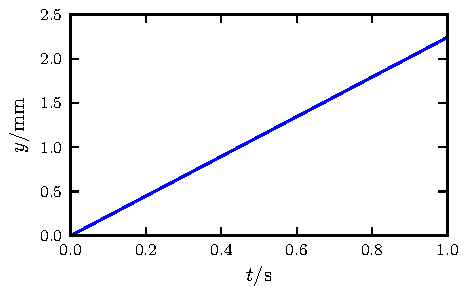
\includegraphics{../code/eCrossBTestY.pdf}
\caption{Drift along $y$ due to crossed magnetic and electric fields.}
\label{fig:driftXY}
\end{figure}

This drift is illustrated in Fig.~\ref{fig:driftXY}.  Note that the step
size in these simulations was $1{\rm ms}$, approximately $10^4$ times
larger than the cyclotron period.  Nonetheless the drift motion is
reproduced accurately.


\subsubsection{Convergence of the integrators}

To study the convergence of the integrators we have taken a crystal with
127 ions and prepared them in a steady state by means of artificial
cooling...
\domcomment{Need to discuss how we find the stationary state of the
  ions}

\domcomment{Make a table of experimental parameters}

We have then integrated the motion of the ions for a total duration of
$10\mu {\rm s}$ using various step sizes for the integrator.  A
reference solution is computed using $\Delta t=10^{-10}{\rm s}$.  In
Fig.~\ref{fig:convergencePlot} we show the mean Euclidean distance
between ions in the reference solution and ions for a given $\Delta t$,
\begin{equation}
\Delta \mathbf{r} = \sqrt{\frac{1}{N}\sum_{j=1}^N(\mathbf{r}_{j,{\rm
    ref.}}-\mathbf{r}_{j,{\Delta t}})^2}\;.
\end{equation}
Note that the ion crystal rotates by nearly $\pi$ radians during $10\mu
s$.  The ions near the periphery of the crystal travel approximately
$1{\rm mm}$ during that time.
We show the errors for three different cases: evolution under just the
magnetic field (blue dots); magnetic field and Coulomb repulsion (green
squares); and magnetic field with Coulomb repulsion and electrostatic
trap potential.  As can be seen, the errors in the solution with just a
magnetic field are independent of the time step size up to round-off.
Obviously this is to be expected since we solve that part of the problem
exactly.  When Coulomb repulsion is included the errors are consistent
with round-off up to a time step size of $\Delta t\approx 10^{-8}{\rm
s}$.  For larger time step sizes the errors grow quadratically.  For
$\Delta t\approx 10^{-6}{\rm s}$ the errors become comparable to an
inter-ion spacing.  When
the electrostatic potential is included in addition to the Coulomb
repulsion the errors are consistent with round-off only up to
$\Delta\approx 10^{-9}{\rm s}$ with quadratic growth after that.  The
errors become comparable to an inter-particle spacing at $\Delta
t\approx 10^{-7}{\rm s}$.

The errors do not grow monotonically once $\Delta t$ becomes comparable
to the cyclotron period $T_{\rm cycl.}=1.32\times 10^{-7}{\rm s}$.
Instead the errors are highly structured as is illustrated in the inset
in Fig.~\ref{fig:convergencePlot}.  This is due to a resonance between
the cyclotron motion and the other terms in the Hamiltonian.  For
instance the first peak in the errors at $\Delta t = T_{\rm cycl.}$
arises because e.g. the kick due to the electrostatic potential is
always applied at the exact same phase of the cyclotron oscillation.
Their effects thus add up in a coherent way.  The same phenomenon occurs
for all harmonics of the cyclotron frequency, i.e. when $\Delta t = n
T_{\rm cycl.}$ with $n$ and integer.  In reality the electrostatic
potential acts concurrently with the magnetic field during the entire
period of the cyclotron oscillations.  When the time step size is
slightly increased, the kicks are again applied at different phases of
the cyclotron motion leading to a more accurate integration.   

This observation points to a possible improvement of our integration
scheme.  The key thing that has to be avoided is a resonance between the
cyclotron motion and the kicks.  One way to achieve this is by choosing
$\Delta t$ randomly according to a suitably chosen probability
distribution.  In the present work we do not implement this
modification.  Instead we use small enough step sizes, $\Delta t\lesssim
10^{-8}{\rm s}$.  The reason for this is two fold.  First, for reliable
results we need errors that are small compared to an interparticle
spacing.  Second, larger time steps introduce larger kicks due to laser
cooling.  These larger kicks cause problems with the crystal stability.

\begin{figure}
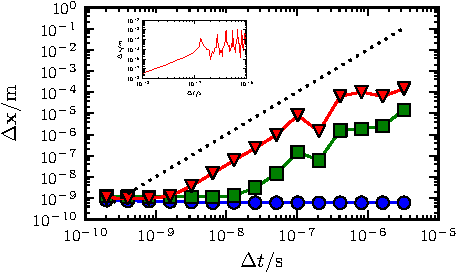
\includegraphics{figures/convergencePlot}
\caption{Convergence of integrators as a function of the time step size
  $\Delta t$.  The blue dots show the errors for evolution under the
    influence of $B_z$ alone.  The green squares include the Coulomb
    repulsion between the ions, and the red triangles include the
    electrostatic potential.  The dashed line has slope 2 and is for
    orientation.  The inset shows a closeup of the errors with magnetic
    field and Coulomb repulsion in the range $1.0e-8 s < \Delta t <
    1.0e-6$.}
\label{fig:convergencePlot}
\end{figure}


\subsection{Simulation of laser cooling}
\label{ssec:laserCooling}

We adopt a very simplistic model of laser cooling which is directly
motivated by the microscopic physics upon which laser cooling based.
This model has the advantage of automatically including both
deterministic damping as well as the fluctuating forces inherent in
laser cooling.  Both of these components of the radiation pressure force
are required by the fluctuation dissipation theorem.  The balance
between them gives rise to the Doppler limit.

We model the internal structure of the ions by two quantum mechanical
levels representing the two states involved in the cycling transition
used for laser cooling.  A two level atom at position $\mathbf{r}$
scatters photons out of a laser beam with wavevector $\mathbf{k}$ with a
rate
\begin{equation}
\dot n (\mathbf{r}, \mathbf{v}) = 
S(\mathbf{r})\frac{\gamma_0}{2\pi}
\frac{(\gamma_0/2)^2}{(\gamma_0/2)^2(1+2S(\mathbf{r}))+\Delta^2(\mathbf{v})}\;,
\end{equation}
where $\gamma_0$ is the natural linewidth of the cycling transition (in
radians per second), $S(\mathbf{r})$ is the saturation parameter, and
$\Delta(\mathbf{v})=\Delta_0 + \mathbf{k}\cdot\mathbf{v}$ is the
detuning of the cooling transition from the laser frequency including
the first order Doppler shift.  We assume that the atoms scatter photons
with this rate with Poissonian number statistics\footnote{Strictly
speaking, this is only valid in the limit of low saturation (for
$S\sim 1$ we have to take into account anti-bunching).}.  We take into
account the beam profile by multiplying the saturation parameter with a
Gaussian factor that accounts for the spatial structure of the laser,
\begin{equation}
S(\mathbf{r})=e^{-\rho^2/\sigma^2}S_0\;,
\end{equation}
where $\rho$ is the distance of the atom from the center of the beam and
$\sigma$ is the $1/e$ radius of the intensity of the beam.

To simulate laser cooling we proceed as follows.  First we compute the
mean number of photons scattered by ion $j$ in time interval $\Delta t$,
\begin{equation}
n_j=\dot{n}_j \Delta t
\end{equation}
The velocities and positions needed for computing $\dot{n}_j$ are taken
at the center of the time step in accordance with the integration scheme
discussed above.  We then compute the actual number of photons scattered
by each ion as a Poissonian random number with mean $n_j$.  Each
particle receives a total momentum kick of 
\begin{equation}
\mathbf{\Delta p}_j = \mathbf{\Delta p_{j,{\rm absorb}}} + 
\mathbf{\Delta p_{j,{\rm emit}}}\;,
\end{equation}
where $\mathbf{\Delta p_{j,{\rm absorb}}}=n_j \hbar \mathbf{k}$ and
$\mathbf{\Delta p_{j,{\rm emit}}}$ is the recoil corresponging to $n_j$
photons scattered in random directions.  To compute $\mathbf{\Delta
p_{j,{\rm emit}}}$ we generate $n_j$ vectors of length $\hbar k$
pointing in random directions.  The recoil momentum $\mathbf{\Delta
p}_{j,{\rm emit}}$ is then obtained by adding up these vectors.

This approach captures the microscopic physics of laser cooling except
for two phenomena.  First, in the case of strong saturation,
$S\gtrsim 1$, quantum statistical phenomena start to play a role.
These manifest themselves in the form of anti-bunching of the photons
scattered in resonance fluorescence.  In essence, there is an
anti-correlation between photon emission events due to the fact that
immediately after a photon emission an atom is in the ground state with
certainty and therefore cannot emitt another photon right away.  This
correction to resonance fluorescence is probably rather unimportant in
the current context, especially because the saturation parameter is not
very much greater than 1.  The other approximation entering our model is
that the photon emission is nearly instantaneous relative to the
dynamics of the ions, i.e. the motion is uniform during an excited
state lifetime,
\begin{equation}
\eta \equiv T_{\rm cycl}(\gamma_0/(2\pi)) \ll 1\;.
\end{equation}
In our case this ratio is approximately $\eta \sim 0.3$.  Furthermore we
have to ensure in the simulations that
\begin{equation}
\Delta t \lesssim S\gamma_0/(2\pi)
\end{equation}
avoid having many photon emission events based on a velocity that was
only realized for a small fraction of the time step.


\section{Free space laser cooling}

As a simple test of our laser cooling model we simulate free space laser
cooling, i.e. the ions are not subject to any trapping or magnetic
fields.  Figure~\ref{fig:FreeSpaceCooling} shows the velocities of 10 Be
ions subject to laser cooling.  The atoms start with a velocity of
$20{\rm m}/{\rm s}$ in the positive $z$ direction.  Two counter
propagating lasers pointed along the $z$ axis irradiate the atoms. The
two counter propagating cooling lasers have peak intensities of $S=0.1$
and are detuned by $0.5\gamma_0$ to the red of the cycling transition at
$313{\rm nm}$.  The atomic linewidth is $\gamma_0=19\times {\rm MHz}$ .
The laser propagating in the $-z$ direction has a beam waist of
$0.01{\rm m}$ and the beam propagating in the $z$ direction has a
uniform intensity profile (i.e. inifinite beam diameter).

As can be seen in Fig.~\ref{fig:FreeSpaceCooling}, the ions are cooled
to the Doppler limit.  Eventually until they diffuse out of the $-z$
beam.  After that they are accelerated by the unbalanced power in the
$z$ direction.  The rms velocity at the Doppler temperature is
\begin{equation}
\sqrt{\langle v_z^2\rangle} = \frac{\hbar \gamma_0}{3 m} \approx
0.25{\rm m}/{\rm s}\;,
\end{equation}
which is in good agreement with our simulations
\domcomment{Should measure our temperature and calibrate}.


\section{Laser cooling of trapped ion crystals}


\subsection{Axial cooling}

Figure~\ref{fig:FreeSpaceCooling} shows the trajectories of 127 ions
subject to axial laser cooling with a saturation parameter of $S=0.1$.

\begin{figure}
\begin{center}
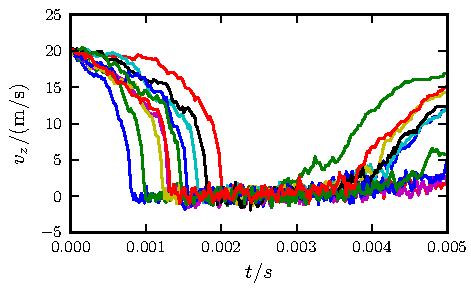
\includegraphics{figures/freeSpaceCooling}
\end{center}
\caption{Velocities of 10 atoms subject to laser cooling.  See text for
details.}
\label{fig:FreeSpaceCooling}
\end{figure}


\subsection{Perpendicular laser cooling}

\begin{figure}
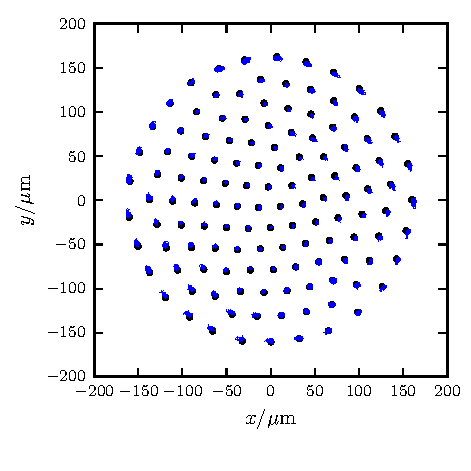
\includegraphics{figures/topView44_115kHzAxial_8ms.pdf}
\caption{Top view of ion crystal subject to axial cooling only over a
  period of 8ms.}
  \label{fig:ionTrajectoriesAxial}
\end{figure}


\subsection{Perpendicular and axial laser cooling}

\begin{figure}
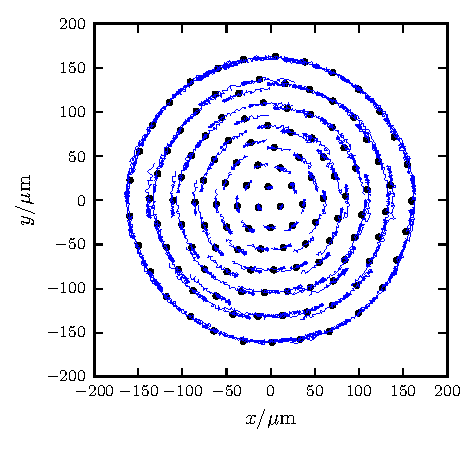
\includegraphics{figures/ionTrajectories_PerpCooling}
\caption{Top view of ion crystal subject to perpendicular cooling only over a
  period of 10ms.}
  \label{fig:ionTrajectoriesPerp}
\end{figure}

\begin{figure}
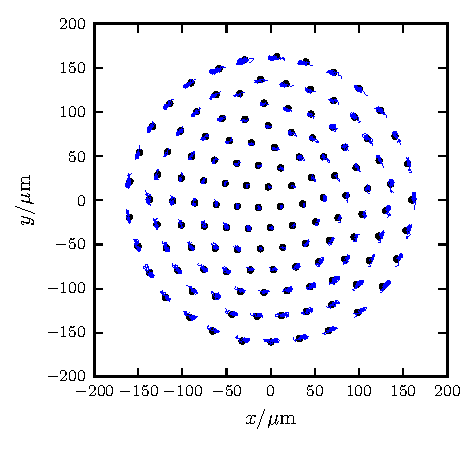
\includegraphics[width=0.49\textwidth]{figures/topView44_10875kHzPerpAxial_5ms}
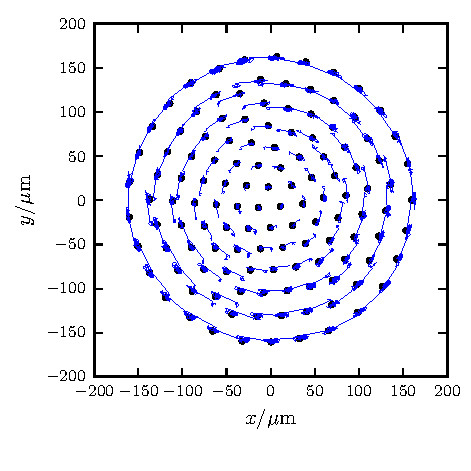
\includegraphics[width=0.49\textwidth]{figures/topView44_10875kHzPerpAxial_6ms}
\caption{Top view of ion crystal subject to both perpendicular and axial
  cooling over a period of 10ms.}
  \label{fig:ionTrajectoriesAxialPerp}
\end{figure}

\section{Follow up}

It turned out that I had a sign mistake in the rotation frequency
of the rotating wall potential.  As a consequence the rotating wall
potential averaged to zero and I got confinement of the ions merely due
to the artificial cooling of their angular motion.  This manifested
itself in nearly circular ion distributions for trap asymmetries (the
    parameter $\delta$) for which the crystal should be highly
elliptical.  In addition I saw large angular drifts (see Fig. 3,4).

After fixing the sign in the rotating wall potential I repeated the
numerical experiment where I cool the ion motion with both axial and
perpendicular laser cooling.  To this end I prepare an initial state
using the artificial cooling (i.e. without noise and in the rotating
    frame).  I chose a cooling rate for the angular velocity of
$\kappa_\theta=10^8/s$ (i.e. the angular velocity relaxes to the ideal
    angular velocity $r\omega_W$
    with a rate of $\kappa_\theta$) and $\kappa_z=10^7/s$ for the axial
motion.  The rotating wall potential is turned on with $\delta=0.01$. I
have $\omega_W/(2\pi)=44{\rm kHz}$ and $B=4.458{\rm T}$.  After about 10ms of
evolution with a time step size of $\Delta t =1{\rm ns}$ the ions
settle into an elliptical crystal with an aspect ratio similar to the one
predicted by the Freericks group's code, see
Fig.~\ref{fig:FreericksCodeCrystal}.  There are still some differences
between the Freericks ion configuration and the configuration I see in my
simulations.  For instance the outermost shell contains 32 ions in my
simulations while it contains 34 ions in the Freericks calculation.
It's possible that my configuration would have settled into the
Freericks configuration had I taken the simulations out further.
It's also possible that the simulation is stuck in a local energy minimum.

\begin{figure}
\center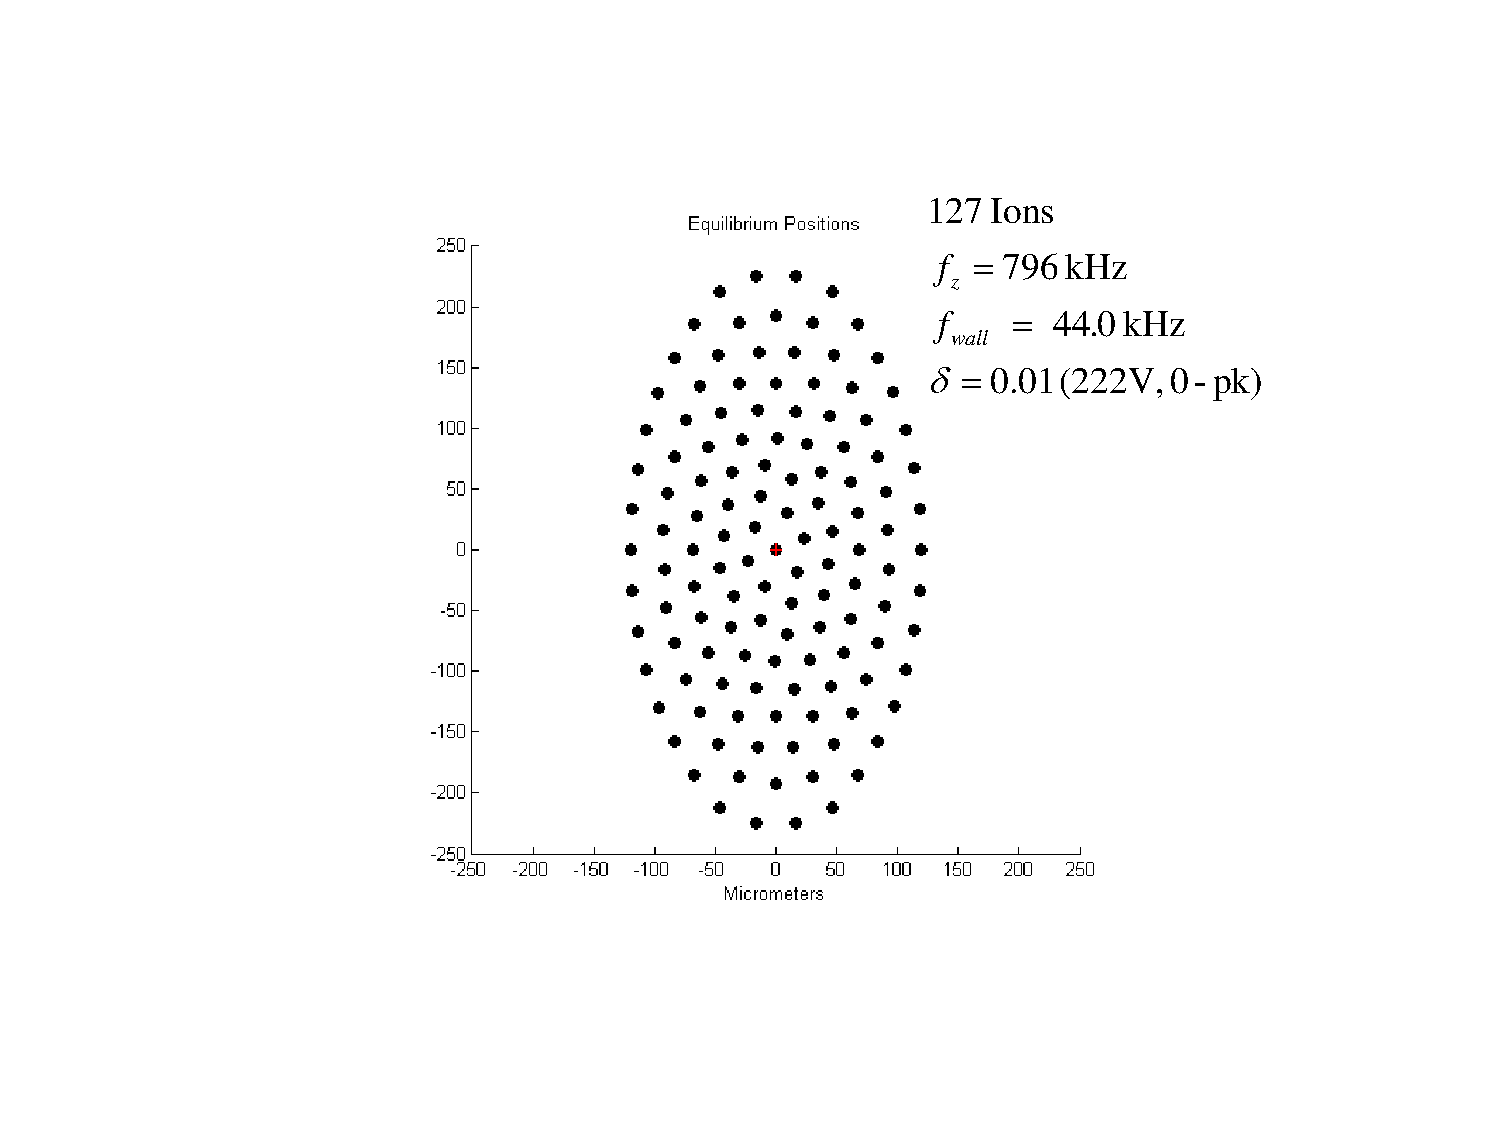
\includegraphics[width=0.95\columnwidth]{figures/Crystal_Configuration}
\caption{Stationary crystal configuration as determined by Freericks
  group's code for 127 ions with $\delta=0.01$.}
  \label{fig:FreericksCodeCrystal}
\end{figure}

After the initial state has been prepared I switch off the artificial
cooling and I switch on the physical laser cooling process described
earlier in these notes.  Currently this involves writing the simulation
state to a file and re-initialize the simulations.  A complication with
that is that I need to restart the rotating wall potential with the
right phase.  Otherwise the crystal starts out at an angle with the
rotating wall potential.  The rotating wall potential then induces large
scale coherent motion which is eventually converted into heat.
In practical terms this prevents me from getting a crystal.

To avoid this a manually tweak the phase of the wall potential until the
crystal and the potential are lined up with one another.  The intial
state of the crystal at this point in the simulations is indicated by
the green dots in Fig.~\ref{fig:ionDynamicsAxialPerp}.

I follow the dynamics of the ions for a total of $1{\rm ms}$ with a time step
size of $\Delta t=1{\rm ns}$.  The path that the ions trace out during
this time is indicated by the black lines.  The final positions are
indicated by the red dots.  The dynamics is somewhat easier to
understand by looking at a movie.  Two horizontal lines of ions just
below the center of the crystal start moving to the left.  Eventually a
few ions take up the vacencies generated by moving an entire
inter particle spacing.  They eventually end up in the starting
positions of their neighbouring ions.  This whole process takes almost 1
ms.  It involves collective motion of the ions.  Each ion by itself
cannot move much.  Instead several ions have to cooperate in order to
find a lower energy state.

Note that with the sign of the rotating wall potential fixed the ion
crystal is rather stationary in the rotating frame.  I do not see the
large overall drifts anymore.

This simulation took about 1.5h on my laptop.  I'm hoping to tweak the
various parameters for the numerical integration to make this go faster.
There are several low hanging fruits in terms of optimization.  In terms
of physics I'd like to look at smaller values of $\delta$ as discussed
per email.  I'd also like to repeat the numerical experiment with only
parallel cooling or only perpendicular cooling.  Then there is the
experiment of moving the perpendicular cooling laser off center.
Presumably these will require that I take the simulations out further.

\begin{figure}
\center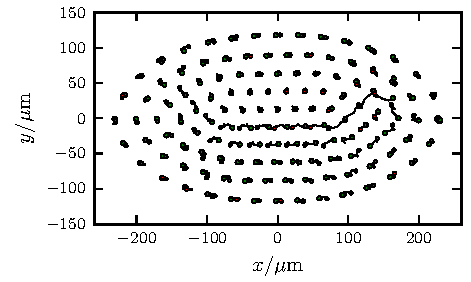
\includegraphics[width=0.95\columnwidth]{figures/rearrangement}
\caption{Dynamics of ion crystal over $1ms$ with parallel and
  perpendicular laser cooling.}
\label{fig:ionDynamicsAxialPerp}
\end{figure}
\begin{itemize}

\item Laser cooling derives from mechanical effects of light in the
course of resonance fluorescence.

\item Model it in a stochastic way.

\item Because the ions have a large velocity spread in the lab frame due
to the rotation of the crystal we have to account for large Doppler
shifts.  Take realistic lineshape into account.

\item Probability for photon scattering given by

\item This is appropriate if the excited state lifetime is short
compared to the cyclotron period.  This is not exactly fulfilled in our
case.  We have to improve on this in the future.  E.g. stochastic
wavefunction trajectories.

\item This gives rise to damping, radiation pressure forces (torque on
    crystal) and fluctuations, all of which are important for the
static and dynamic properties of the crystals.

\item Validation Look at free space cooling, reproduce Doppler
temperature

\item Validation: Look at axial temperature of ions in trap.  Both
agree.

\end{itemize}


\subsection{Convergence of the integration scheme}
\label{ssec:convergence}

In figure \ref{fig:ConvergenceWithDamping} I show the convergence of our
integrator as a function of the time step size.  That figure shows the
mean error in the position of 400 ions after $0.1ms$.  This corresponds
to several periods of the rotating wall potential.  The trap parameters
are the same as in Fig.~\ref{fig:SteadyState}.  The ions are propagated
until steady state is reached.  From that point on we integrate for
another 0.1ms with varying step sizes.


\section{Static crystal analysis}
\label{sec:static}

This is mostly validation work, i.e. trying to convince ourselves that
we're getting things right by comparing against well understood
experimental data and Freericks group's theory.

\subsection{Aspect ratio as a function of rotating wall potential
  strength}

\subsection{1-2 plane transition}

\begin{figure}
\center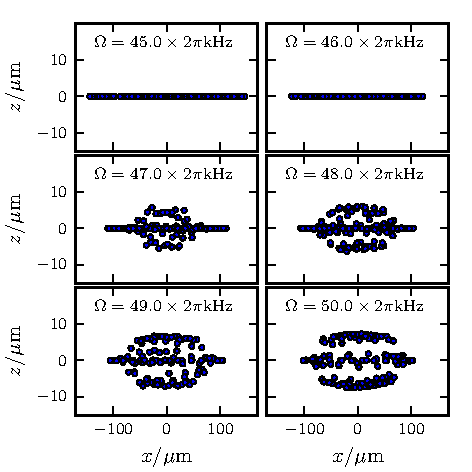
\includegraphics{./figures/sideViews.pdf}
\caption{Side view of the ions in steady state for different rotation
  frequencies.  At $\Omega\approx 50\times 2\pi {\rm kHz}$ the single
    plane configuration becomes unstable.}
\label{fig:SideViewsForVariousOmegas}
\end{figure}

\begin{figure}
\center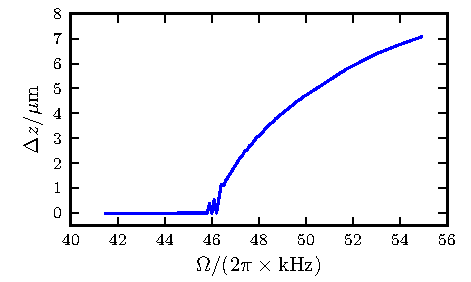
\includegraphics{./figures/thicknessVsOmega.pdf}
\caption{Thickness of the ion crystal as a function of $\Omega$}
\label{fig:ThicknessVsOmega}
\end{figure}

\subsection{Crystal symmetry}


\section{Phonon dynamics, spectra, temperatures, etc.}
\label{sec:dynamics}

\subsection{Spectra}

- Comparison with Freericks group.

- Excitation level, $<n_i>$, etc.

- Mode structure

\begin{figure}
\center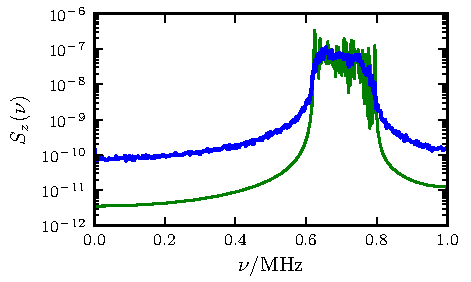
\includegraphics{./figures/axialSpectra}
\caption{Axial spectra.  The green line is without cooling and the blue
  line is with continuous cooling during the recording of the spectrum.}
  \label{fig:axialSpectra}
\end{figure}

\begin{figure}
\center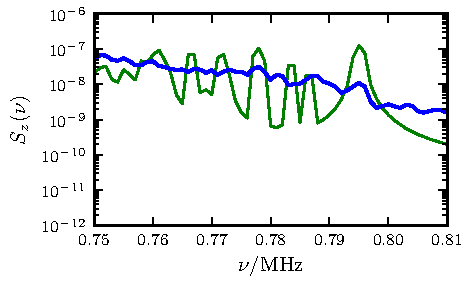
\includegraphics{./figures/axialSpectraZoomedIn}
\caption{Axial spectra.  The green line is without cooling and the blue
  line is with continuous cooling during the recording of the spectrum.
The highest modes (especially the com mode) are visible. }
  \label{fig:axialSpectraZoomedIn}
\end{figure}

\begin{figure}
\center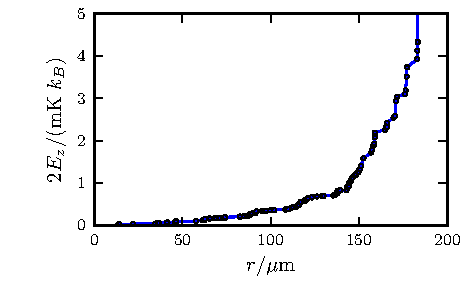
\includegraphics{./figures/axialTemperature}
\caption{Axial temperature as a function of disctance from center of
  crystal.  }
  \label{fig:axialTemperatures}
\end{figure}



\section{Stability of crystal}
\label{sec:stability}

- Excursions of ions as a function of perp cooling beam width,
  displacement from trap center; can do this spatially resolved (i.e.
      are certain regions of the crystal "hotter" than others)

- Frequency of rearrangements; nature of rearrangements.


\section{Investigate other cooling configurations}

- E.g. counterpropagating cooling beams



\section{Conclusion}
\label{sec:conclusion}




\end{document}

